\documentclass[10pt,letterpaper]{article}
\usepackage[left=1.8cm, right=1.8cm, top=1cm]{geometry}
\usepackage[utf8]{inputenc}
\usepackage[T1]{fontenc}
\usepackage[spanish]{babel}
\usepackage{amsmath}
\usepackage{amsfonts}
\usepackage{amssymb}
\usepackage{graphicx}
\usepackage{subfigure}
\usepackage{steinmetz}
\usepackage{float}
%\usepackage{circuitikz}

\author{Clase Práctica $\#$3}
\title{Electrónica I}
\date{Análisis nodal y de mallas}

\renewcommand{\sin}{\sen}
\begin{document}
	\maketitle
	
Bibliografía: Análisis de circuitos en ingeniería. Hayt \textit{et al.} 8va ed. Capítulo 4
\\
 
 1- Usando análisis de nodos o de mallas, determine la tensión marcada como $v_x$ en el circuito representado en la figura. 
 
 b) ¿A qué valor se debe cambiar la fuente de 2 A para reducir $v_x$ en 10\%?
 
  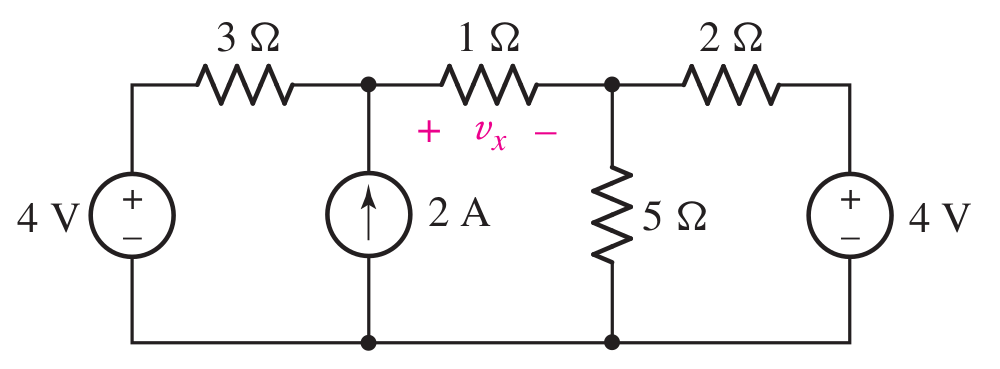
\includegraphics[scale=0.25]{c1}
  
  \textbf{Nota:} Este circuito ya fue analizado en la cp \# 2 en el ejercicio 6 utilizando superposición.
  \\
  
  	2- Usando el nodo inferior como referencia, determine la tensión a través de la resistencia 5 $\Omega$ en el circuito de la figura y calcule la potencia disipada por la resistencia de 7 $\Omega$.
  	
  	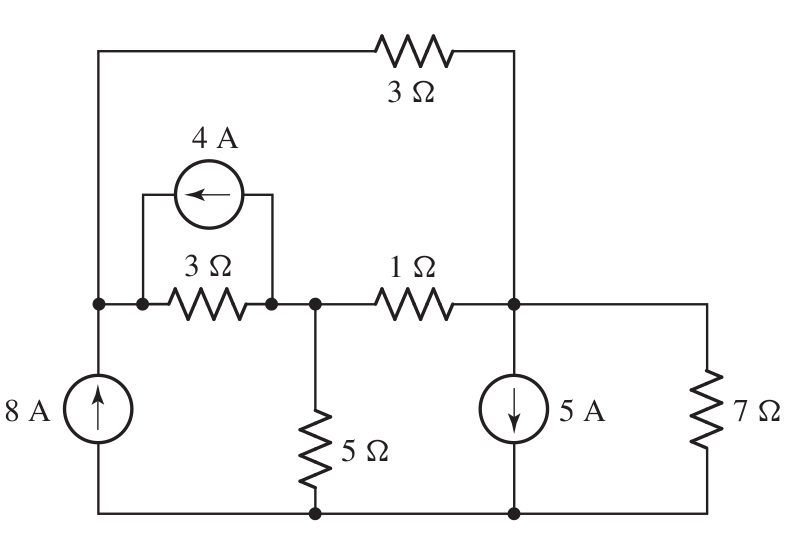
\includegraphics[scale=0.3]{c2}		
  	
  	3- Para el circuito de la figura, determine tensiones de nodo.
  	
	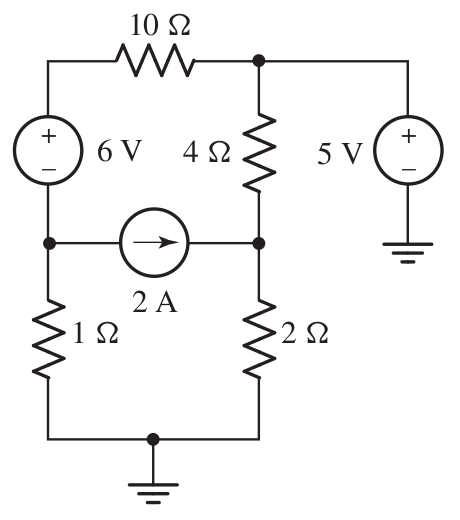
\includegraphics[scale=0.3]{c3}
	
	4- Determine los valores numéricos para cada una de las tres corrientes de malla marcadas en el diagrama de circuito de la figura.
	
		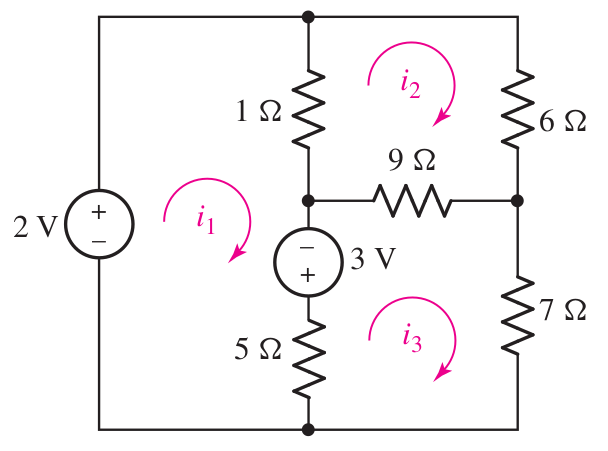
\includegraphics[scale=0.38]{c4}
	
	5- Usando procedimientos de análisis de mallas, obtenga el valor para la corriente marcada como $i$ en el circuito representado por la figura.
	
	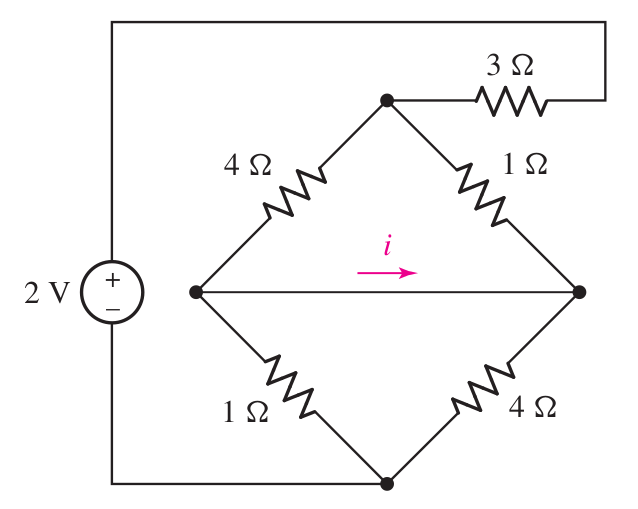
\includegraphics[scale=0.38]{c5}

 	6- Para el circuito de la figura, determine la corriente de malla $i_1$ y la potencia disipada por la resistencia de 1 $\Omega$.
 
 	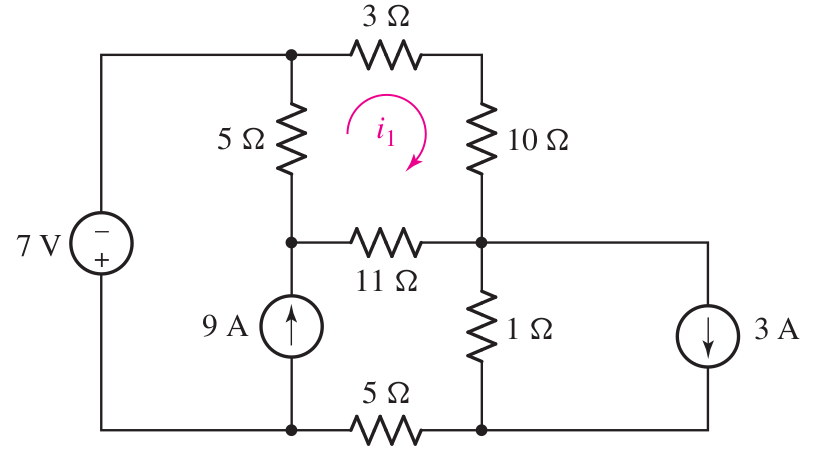
\includegraphics[scale=0.38]{c6}
\end{document}